\documentclass[12pt]{article}
\usepackage[francais]{babel}
\usepackage[utf8x]{inputenc}
\usepackage{amsmath}
\usepackage{graphicx}
\usepackage{float}
\usepackage{dsfont}
\usepackage{amsfonts}
\usepackage[T1]{fontenc}
\usepackage[colorinlistoftodos]{todonotes}
\usepackage{listings}
\usepackage{csquotes}
\usepackage{minted}
\usepackage{hyperref}
\usepackage{ragged2e}
\usepackage[linesnumbered,ruled,french,onelanguage]{algorithm2e}
%tikz 
%dia
\justifying
\newcommand{\deriv}{\mathrm{d}}
\usepackage[margin=3.5cm]{geometry}
\lstset{
    language=Java,
    basicstyle=\scriptsize\ttfamily,
    commentstyle=\ttfamily\color{red},
    numbers=left,
    numberstyle=\ttfamily\color{blue}\footnotesize,
    stepnumber=1,
    numbersep=5pt,
    backgroundcolor=\color{white},
    showspaces=false,
    showstringspaces=false,
    showtabs=false,
    frame=single,
    tabsize=2,
    captionpos=b,
    breaklines=true,
    breakatwhitespace=false,
    title=\lstname,
    escapeinside={},
    keywordstyle={},
    morekeywords={}
}
    
\begin{document}

\begin{titlepage}

\newcommand{\HRule}{\rule{\linewidth}{0.5mm}} % Defines a new command for the horizontal lines, change thickness here

\center % Center everything on the page
 
%----------------------------------------------------------------------------------------
%	HEADING SECTIONS
%----------------------------------------------------------------------------------------

\textsc{\LARGE Université de Caen}\\[1.5cm] % Name of your university/college
\includegraphics[scale=1.2]{LOGO-UNICAEN_V-2.1-N.png}\\[1cm] % Include a department/university logo - this will require the graphicx package
\textsc{\Large Conception logicielle avancée}\\[0.5cm] % Major heading such as course name
\textsc{\large L2 - Informatique}\\[0.5cm] % Minor heading such as course title

%----------------------------------------------------------------------------------------
%	TITLE SECTION
%----------------------------------------------------------------------------------------

\HRule \\[0.4cm]
{ \huge \bfseries Livres dont vous êtes le héros}\\[0.4cm] % Title of your document
\HRule \\[1.5cm]
 
%----------------------------------------------------------------------------------------
%	AUTHOR SECTION
%----------------------------------------------------------------------------------------

\begin{minipage}{0.6\textwidth}

\begin{flushleft} \large
\center
\emph{Auteur:}\\
Nathan \textsc{SAKKRIOU} - 22003438\\ % Your name
Yanis \textsc{HABAREK} - 22010593\\
Alan \textsc{LECOT} - 22003887
\end{flushleft}
\end{minipage}\\[1.5cm]

{\today}\\[2cm] % Date, change the \today to a set date if you want to be precise

\vfill % Fill the rest of the page with whitespace
\end{titlepage}

% Page Remerciements
\mbox{}
\section{Remerciements}
Nous souhaitons adresser nos remerciements les plus sincères à Monsieur Gamblin Sebastien pour son aide apportée, grâce à qui nous avons pu mener à bien ce projet ainsi que le rapport associé.\\
Nous remercions également Monsieur Bonnet Gregory, pour les explications et directives données lors des cours magistraux.\\

A tous ces intervenants, nous présentons nos remerciements, notre respect et notre gratitude.

\newpage
\tableofcontents
\newpage

% DOCUMENT

\section{Introduction} % Fini %
Pour les étudiants en informatique, la programmation orientée objet apparaît comme un passage obligatoire. Ainsi, afin d’en appliquer les principes et de parfaire notre maîtrise de Java, des projets nous ont été proposés dans le cadre de l’unité d’enseignement de TPA (Travail Personnel Approfondi). Par groupe de 4, il nous a été demandé de réaliser des applications complètes, sur différents thèmes : jeux vidéos, sténographie, etc.
Parmi ces propositions, si plusieurs ont retenu notre intention, une, plus que les autres, a
capté notre intérêt : le livres dont vous êtes le héros.\\

Pour comprendre ce que cette notion signifie, nous allons nous appuyer sur la définition que nous donne la page Wikipédia de  \href{https://fr.wikipedia.org/wiki/Un_livre_dont_vous_%C3%AAtes_le_h%C3%A9ros}{\underline{Un livre dont vous êtes le héros}} :
\begin{displayquote}
	Ce nom désigne par extension la catégorie de livre-jeu basé sur le principe présent dans cette collection, d'une progression de lecture en fonction des choix et du résultat des actions du lecteur joueur.\\
	{\small source : \href{https://fr.wikipedia.org/wiki/Un_livre_dont_vous_%C3%AAtes_le_h%C3%A9ros}{\underline{Wkipédia}}}
\end{displayquote}

\section{Objectif du projet} % A compléter %
L'intérêt de rendre ce type de jeu virtuel, est de pouvoir ajouter de nombreuses fonctionnalité dans la personnalisation et dans l'expérience de jeu.\\

Dans notre cas, nous avons développés 3 grandes fonctionnalités nous ont été demandés :\\

\begin{itemize}
    \item Une interface de création/modification d'un livre. Un utilisateur pourra alors créer sa propre histoire, et l'enregistrer afin de pouvoir y jouer ou de la partager.\\
    \item Des algorithmes permettant de calculer différentes informations sur chaque arbre ( comme la difficulté, ou la création du graph d’un arbre ).\\
    \item Une interface de jeu, interprétant un arbre afin de permettre à l’utilisateur de naviguer dedans en fonction de ses choix.\\
\end{itemize}

Au cœur de ses 3 grandes fonctionnalités nous avons implémenter une multitude d'aspect, améliorant l'expérience, livres dont vous êtres le héros version papier. Elles vont être dévoilées et expliquées par la suite.\\

Il est très important de noter que notre jeu n'est absolument pas optimisé pour l'expérience utilisateur, c'est à dire que, par exemple, dans le cas des monstres, leurs statistiques ne sont équilibrés entre eux, même chose pour les items. Nous avons préférer mettre l'accent sur la possibilité de jouer et les sur les créateur de livres, que sur l'expérience joueur.

\section{Organisation du projet} % A compléter %
Nous avons fait le choix d’organiser notre projet avec une architecture MVC ( Model Vue Controller ).\\

Pour faire très simple, cette organisation en 3 axes permet de diviser son code pour le rendre clair et le maintenir facilement.\\

\begin{itemize}
    \item Le Model représente toute la partie logique de l’application.\\
    \item La Vue désigne, dans notre cas, la classe qui crée et place tout les composants graphiques swing sur une fenêtre.\\
    \item Et le Controller, permet de faire le lien entre les interactions de l’utilisateur ( ex : un clic sur un bouton ) et les informations du Model, et grâce à cela de faire une interface graphique qui s’adapte à un Model.\\
\end{itemize}

Notre projet ou package principal nommé livre, est composé de 5 sous-packages :\\
\begin{itemize}
    \item game`: Regroupe toute les classes du Model.\\
    \item graphics` : Regroupe toutes les Vues et les Controllers ( ceux-ci sont stockés dans un sous-sous-package `controller` ).\\
    \item `algorithm` : Regroupe les classes et méthode de parcours de graphe.\\
    \item `graphview` : Utilise la librairie externe `jung2` pour créer un graph.\\
    \item `unittest` : Regroupe tous les tests unitaires.\\
\end{itemize}

\section{Interface de création / modification d'un livre}
Nous commençons par détailler l'interface de création d'un livre, appelé Template Creator dans la page d'accueil. En effet il nous permet d'abord de comprendre notre représentation d'un livre, avec ses scènes et ses interactions, informations qui nous seront utiles pour mieux appréhender le fonctionnement de l'interface de jeu.

\subsection{Représentation d'un livre}
Sachant qu'il existe de nombreuses approches de livre pour ce genre de programme, il nous a donc fallu choisir notre propre représentation.\\
Selon nous un livre, est composé de :

\begin{itemize}
    \item Une scène de départ
    \item Une scène d'arrivée
    \item Une quantité d'or et un objet à obtenir pour gagner la partie
    \item Au moins un bloc regroupant des scènes avec des interactions aléatoire
    \item Un nombre de répétition des blocs de scènes\\
\end{itemize}

Nous continuerons à expliciter les définitions de ces éléments par la suite.

\begin{figure}[h]
    \centering
    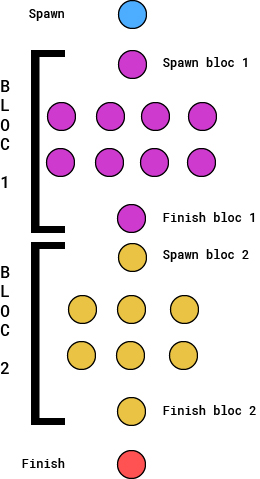
\includegraphics[scale=0.5]{exemple_tree.jpg}
    \caption{Exemple de la forme type d'un livre}
\end{figure}

\subsubsection{Scène et interaction}
Ainsi nous comprenons assez vite qu'un livre peut être représenté comme un arbre, où chaque noeud est une scène. Le joueur se déplacera de scène en scène en fonction de ses choix.\\
Pour comprendre la composition et la forme d'une scène, nous allons nous intéresser à la représentation en JSON d'une scène.\\

\begin{listing}[h]
\begin{minted}[frame=single,
               framesep=3mm,
               linenos=true,
               xleftmargin=21pt,
               tabsize=4]{js}
{     
    "name": "Grotte",
    "alias": "cave",
    
    "interaction": {
        "item": "key",
        "type": "foundItem"
    },
    
    "nextScene": [
        19, 20, 21
    ],
    
    "id": 25
}
\end{minted}
\caption{JSON d'une scène} 
\end{listing}

Tout d'abord, `name` représente la nom de la scène, celui qui va être afficher.\\\\
`alias` est un slug de `name`, qui va nous permettre de rechercher plus facilement une scène.\\\\
`interaction`, point très important, une interaction représente ce qu'il va se passer dans la scène, l'interaction avec le joueur. On en compte, dans le jeu de base, 9 différentes citées ci dessous.

\begin{center}
\begin{tabular}{ c c }

Text & Permet d'afficher du texte pour raconter une histoire\\ 
Final & Désigne la scène de fin, et permet également d'afficher du texte\\  
GameOver & Le joueur tombe dans un piège et la partie s'arrête\\
Battle & Combat contre un monstre\\
Shop & Permet d'acheter des objets pour améliorer ses statistiques\\
Temple & Ici le joueur récupère tous ses points de vie\\
FoundItem & Le joueur récupère trouve un objet par terre, et l'ajoute a son inventaire\\
Treasure & En échange d'une clé, le joueur ouvre un coffre, et récupère un objet\\
Null Interaction & Permet de créer une scène sans interaction\\
\end{tabular}
\end{center}

Dans le code toutes ces interactions implémentent une interface

\begin{listing}[h]
\begin{minted}[frame=single,
               framesep=3mm,
               linenos=true,
               xleftmargin=21pt,
               tabsize=4,
               ]{js}
package livre.game.scene;
import org.json.simple.*;


public interface Interaction {

    public String getType();
    public JSONObject toJSONObject();
}
\end{minted}
\caption{Interaction.java} 
\end{listing}

La méthode `getType()` permet au controller (que l'on reverra un peu plus tard) d'adapter ce qu'il doit faire en fonction de l'interaction de la scène où le joueur se trouve.\\

\textit{Première fois que nous rencontrons une méthode `toJSONObject()`, à noter que nous utilisons cette méthode dans de nombreuses classes afin de faciliter la mise en fichier de notre modèle, par exemple, pour la sauvegarde d'une partie complète, il suffit juste d'appeler les méthodes de `toJSONObject()` de chaque élément pour avoir un fichier de sauvegarde complet sous format JSON}\\

Nous trouvons ensuite `nextScene`, une liste d'entier, ces entiers représentes les `id` d'autres scènes, des scènes suivantes. Cet attribut correspond au numéro de la scène, et permet de facilement naviguer entre elles.

Nous avons passé en revu tous les concepts que compose la structure de scène et les avons adaptés en java (Voir code). Un livre, est donc une liste de scène, dans notre cas une `ArrayList`de type `Scene`.

\subsubsection{Template de livre}
Nous avons vu comment un livre était représenté dans notre programme, mais il serait encore trop compliqué sur le long terme d'être obligé de créer chaque scène une par une, en effet un livre dont vous êtes le héros peut contenir des centaines de pages. 
Nous avons donc pensé à un format de fichier qui correspondrait à un moule de livre, un template de livre. Ce fichier, bien plus court, en JSON, contiendrait toutes les informations cité précédemment, et un algorithme transformera se fichier en une `ArrayList` de `Scene`.\\


\begin{figure}[h]
    \centering
    \includegraphics[scale=0.75]{Capture.PNG}
\end{figure}


Nous avons ici un template basique, et si nous le regardons bien, nous voyons tout les points cité précédemment, une scène de départ et d'arrivée, un objet et une somme d'or en objectif pour la fin de la partie, et un gros morceau correspondant au bloc que nous allons détailler ici.\\
Si on regarde le schéma nous pouvons apercevoir qu'un bloc est composé d'une scène d'entrée et une scène de sortie, et entre les deux, plusieurs scènes. Plus clairement, un bloc est composé de :\\

\begin{itemize}
    \item Un point de départ du bloc | `start\_node`.
    \item Un point de fin du bloc | `end\_node`.
    \item Un nombre de répétions de chaque ligne du bloc | `nbRepeat`.
    \item Une liste de nom et d'alias de scène qui apparaîtront sur chaque ligne | `nameBetween`.
    \item Une liste d'interactions qui seront aléatoirement distribuées aux scènes précédemment citées | `possibleInteraction`.\\
\end{itemize}

Le fonctionnement d'un bloc est simple, on place le point de départ et de fin a chaque extrémité, et entre les deux, on crée un nombre de ligne correspondant à `nbRepeat`. Dans chacune de ces lignes, on crée et on ajoute les scènes possibles depuis le nom et l'alias noté dans `nameBetween`, pour finir, les interactions contenues dans `possibleInteraction` sont attribuées aléatoirement à chaque scène.\\

L'attribut bloc, est une liste, et donc, même si dans notre exemple, nous n'avons qu'un bloc, il est possible d'en avoir autant possible.

\subsubsection{Algorithme de création de livre grâce à un template}
Nous avons maintenant compris la structure d'un livre et d'un template de livre, notre objectif maintenant est de passer d'un template à un livre afin de l'utiliser dans le jeu. Les 3 méthodes qui nous intéresse sont implémentés dans la classe `TreeGenerator`, elles sont appelés :

\begin{center}
\begin{tabular}{ c c }

`loadTreeWithTemplate` & Depuis le path d'un template, renvoie une\\
&`ArrayList` de `Scène`\\
`createRandScene` & Avec toutes les informations d'un bloc créé \\
& le bloc et renvoi une `ArrayList` de `Scène`\\
`LoadNodeTree` & Charge et crée une scène
\end{tabular}
\end{center}

Le gros de ces fonctions est de la récupération d'information depuis le JSON du template et d'appliquer le bon typage aux informations, la seule partie intéressante est la création d'un bloc, donc de la méthode `createRandScene`. Nous allons expliquer et comprendre cet algorithme.\\

Il y a 3 choses importantes dans cet algorithme :\\
\begin{itemize}
    \item Il faut créer les scènes
    \item Attribuer les interactions aléatoirement
    \item Ajouter les bons id de scène dans les `nextScene` afin de connecter correctement les scènes entres elles.\\
\end{itemize}
Pseudo-Code de createRandScene:
\begin{lstlisting}
ArrayList<ArrayList<Scene>> data = new ArrayList<>()

// Creation des scenes avec interaction
for(int i = 0; i < nbRepeat; i++){
    ArrayList<Scene> row = new ArrayList<>();
    for(int j = 0; j < aliasList.length; j++){
        Scene scn = new Scene(nameList[j], aliasList[j])
        int index = 0 <= randomInt <= nbInteraction
        Insere l interaction a la scene
        row.add(scn)
        tree.add(scn)
    }
    data.add(row)
}

// Connexion des nextScene entre les scenes
for(int i = 0; i < data.length - 1; i++){
    for(Scene top : data.get(i)){
        for(Scene bot : data.get(i+1)){
            top.addNextScene(bot.getId())
        }
    }
}

// Connexion de la premiere ligne avec le premier noeud
for(Scene firstRow : data.get(0)){
    startNode.addNextScene(firstRow.getId())
}

// Connexion de la derniere ligne avec le dernier noeud
for(Scene lastRow : data.get(data.size()-1)){
    lastRow.addNextScene(endNode.getId())
}
\end{lstlisting}

\textit{\\A noter que les id des scènes sont définies en statiques, et sont incrémentés automatiquement à chaque instanciation.}
\newpage
\subsection{Interface graphique}
Nous avons détaillés et compris tous les types de données nécessaire a la représentation d'un livre (livre, template de livre, scène, interaction), maintenant nous allons nous intéresser à l'interface qui permettra à un utilisateur de créer son propre template de livre.\\

Tout d'abord, nous avons le choix entre créer ou modifier un template, la différence entre les deux c'est juste que tout les champs de saisie seront pré entré si l'on choisie l'option modifier, sinon, tout les champs seront vide.\\

Tout les champs seront dispatchés dans différents onglets : \\
\begin{figure}[h]
    \centering
    \includegraphics[scale=0.45]{template_creator.PNG}
\end{figure}

Les quatre premières onglets correspondent à tout ce qui est nécessaire pour la création d'un template de livre, les deux suivants, Algorithme et Visualisation, permettent d'obtenir des informations sur un arbres (ces algorithmes seront détaillé un peu plus tard).\\

Tout les champs sont relativement simples à compléter, et dès lors que ces quatre champs sont remplis, il est possible d'enregistrer son template, qui arrivera sous la forme d'un JSON dans le dossier `custom\_template`, toutes les difficultés possibles dans la complétion des champs sont détaillées dans la documentation. Via le bouton ouvrant la page web des informations principales.

\section{Interface de jeu}
L'interface de jeu se base sur le modèle, pour comprendre son fonctionnement, et comme dit précédemment, tout notre modèle se trouve dans le dossier `game`, et plus précisément dans le dossier `player`. Une fois que l'on aura compris toutes les subtilités de notre modèle, l'interface graphique n'aura plus qu'à adapter, sous forme de texte dans notre cas, l'état du modèle.

\begin{figure}[h]
    \centering
    \includegraphics[scale=0.50]{packages.png}
\end{figure}
\newpage
\subsection{Modèle}
Nous avons fait le choix de centraliser tout notre modèle au sein d'une seule classe, dans notre cas `Player`. Le `Player` contient tout ce qui est nécessaire pour le jeu, c'est à dire l'arbre de jeu, et toutes les statistiques du joueur. Nous voyons sur le diagramme ci-dessous toutes les classes qui composent notre modèle.\\

Pour nous faciliter la tâche, nous avons utilisé une collection de données qui nous provient de ce  \href{https://www.npmjs.com/package/pokemon-assets}{site}. Tous un tas d'information sur les pokémons, leurs compétences, les objets etc sont rassemblé dans des fichiers JSON. Nous avons récupérer les informations sur les 3 sujets cités précédemment et nous les avons adapté à notre usage, ces fichiers se retrouvent dans le dossier `data` sous les noms :\\
\begin{itemize}
    \item monsters.json
    \item items.json
    \item skills.json
\end{itemize}

\subsubsection{Fighter, Monstre, Skill et Item}
Nous retrouvons tout en haut de ce schéma une classe `Fighter`, elle regroupe tous les attributs et les méthodes permettant de modéliser un combattant, qui peut subir des dégâts, et utiliser des skills pour en infliger, cette classes nous la faisons hériter au player et au monstre, cela sera utiles pour l'interaction `Battle`, qui représente un combat player vs monstre. De plus on retrouve la méthode `toJSONObject()` qui va permettre, pour le joueur surtout, de sauvegarder ses statistiques dans un fichier de sauvegarde.\\

La partie intéressante sur les skills, déjà, ils ont une valeur de dégât qu'ils infligerons mais également un taux de succès, c'est une valeur de 0 à 100 qui désigne le taux de réussite d'une compétences. Dans le code, cela se traduit dans la méthode `useSkill()`. Un entier de 0 à 100 est tiré aléatoirement, et si celui ci est inférieur ou égal à la valeur du taux de succès du skill, les dégâts sont infligés, dans le cas contraire, 0 dégât sont infligés. Dans le cas du player, les skills utilisé seront choisi par l'utilisateur, et dans le cas d'un monstre, il seront tiré aléatoirement.\\

Dans le cas des montres les skills sont attribués aléatoirement depuis la liste des compétences disponibles du fichier monsters.json, dans leur objets attribués.\\

Une notion très importante de notre modèle, qui va nous faciliter grandement la tâche, ce sont les classes `EveryItem`, `EverySkill` et `EveryMonster`. Ces classes vont nous permettre à l'initialisation, de lire leurs fichiers JSON, d'instancier tous les éléments correspondant et grâce à cela de pouvoir les récupérer facilement grâce à leurs noms, leurs alias ou aléatoirement. 

\subsubsection{Player}
Nous retrouvons la classe 'Player' qui hérite de la classe 'Fighter' vu ci dessus , elle est très importante au niveau du jeux, car en effet tout le modèle est rassemblé au niveau de cette classe.\newline
Elle regroupe toutes les informations importantes sur le joueur comme sont nombre de gold, d'objectif gold et item, ses skills mais aussi la scène actuelle du jeux.
\begin{minted}[frame=single,
               framesep=3mm,
               linenos=true,
               xleftmargin=21pt,
               tabsize=4,
               ]{js}
public void loopItemInInventory(){
        for(Item i : this.inventory){
            this.updateWithItem(i);
            this.checkIfGotObjectiveItem(i);
        }
    }
\end{minted}
On retrouve aussi une méthode permettant de parcourir l'inventaire du joueur (ci-dessus) et d'autres méthodes permettant de mettre a jour les statistiques du joueur avec les items bonus, d'ajouter un item a l'inventaire, de vérifier si je joueur possède l'item objectif dans sont inventaire, et plein d'autres fonctionnalités comme rajouter des sommes d'or au joueur, lui en retirer, et ainsi de suite afin d'avoir un inventaire qui se met a jour en continue en fonction des interactions du joueur.\newline
De plus on retrouve la méthode ‘toJSONObject()‘ qui va permettre, pour le joueur surtout, de sauvegarder sa partie et ses statistiques
dans un fichier de sauvegarde.

\subsection{Interface graphique}
Nous avons vu au plus haut que nous avons organisé notre projet avec une architecture MVC (Model Vue Controller), nous avons déjà parlé du Modèle et de la vue (plus haut) maintenant on se place dans le sous-package \textbf{graphics} dans le sous-sous-package \textbf{controller} pour voir  comment est fait le lien entre les interactions de l'utilisateur et les informations du Modèle.

\begin{center}
    \includegraphics[scale=0.5]{graphics.png}
\end{center}
Nous avons effectivement 4 classes du sous-sous-package controller "ControlHome", "ControlGamePage", "ControltreeChoice", "ControlTemplatePage" afin de controller respectivement les classes Home (qui est le menu du jeux au lancement), GamePage ( qui est l'ui (interface utilisateur) du jeux en pleine partie), TreeChoice (qui permet de choisir entre charger l'arbre de base/personnalisé , TemplatePage(qui permet de crée un template).\newline
Ces classes permettent donc le lien entre le modèle et la vue et d'avoir en même temps un code plus propre et plus indépendant, les méthodes sont appelées dans une classe (par exemple \textbf{GamePage}), et sont définies dans la classe-controller(\textbf{ControlGamePage}) correspondant a la classe , on peut considérer les deux classes sont donc liées.\newline
C'est donc de cette manière que fonctionnes tout les boutons du jeux par exemple les 4 boutons  skills du joueurs qui sont dans une Classe ont leurs méthode ActionListener définies dans une autre classe du sous-sous-package controller(voir ci-dessous).
\begin{lstlisting}
btn.addActionListener((e) -> this.controller.actionSkill1Button(e));
\end{lstlisting}
  	\textit{$\uparrow$on appel la fonction depuis la classe GamePage$\uparrow$}\newline 
\textit{$\downarrow$ définie la méthode dans ControlGamePage                                        $\downarrow$}
\begin{lstlisting}
public void actionSkill1Button(ActionEvent event){
        int idSkill = 0;
        launchSkill(idSkill);
    }
\end{lstlisting}


\section{Graphes, algorithmes et visualisation}
Dans l'optique d'enrichir notre projet, nous avons implémenté différentes fonctionnalités se référant aux graphes, leur visualisation ainsi que les différents algorithmes utilisables.

\subsection{Graphes}
Afin de produire nos implémentations, il nous était important de réfléchir à la notion de graphes informatiques. \\
A l'instar des arbres binaires, les graphes sont des structures de données comprenant des noeuds et des couples de noeuds symbolisant un chemin entre eux. Cependant les graphes ne proposent pas tous de hiérarchie entre les noeuds, ainsi on distingue les graphes non orientés, où les chemins relient deux noeuds dans un sens et dans l'autre, et les graphes orientés, où les chemins appelés flèches ne relient deux noeuds que dans un sens définit. De plus certains chemins peuvent être pondérés afin de représenter la distance entre deux villes par exemple.\\
On remarque alors assez vite que le livre sensé représenter une histoire implique une hiérarchie des événements (en l'occurrence des noeuds) mais que les chemins entre ces noeuds ne représentent pas de distance en soit. Nous avons en ce sens opté pour un graphe orienté non pondéré, où les noeuds deviennent ici des Scènes. Pour cela nous avons produit deux types de graphes orientés non pondérés afin répondre aux exigences de chaque implémentations.

\subsubsection{Le graphe utilisé dans l'algorithme}
Lors de la production d'algorithmes nous avons dans un premier temps réalisé une classe Graph comprenant une liste de chemins entre une Scène et une Scène qui en découle. Cependant nous avons rapidement revu notre méthode car l'une des caractéristiques des scènes et qu'elles contiennent une liste des identifiant d'autres scènes. Ainsi un livre est déjà un ensemble de noeuds comprenant des pointeurs vers d'autres noeuds. Il nous a donc paru évident d'exploiter cet aspect du Livre pour le développement du projet.

\subsubsection{Le graphe utilisé dans la visualisation de graphe}
Toutefois comme nous le verrons par la suite dans la sous-section sur la visualisation du graphe, il nous a fallu créer un graphe correspondant aux attentes de la librairie utilisée. Nous retrouvons alors dans le sous package graphview, la classe SimpleGraphView qui instancie un graphe orienté. Cette classe comprend des Scènes et des chemins ici appelés "Vertex" et "Edge" et est créée comme pour l'algorithme à partir d'un Livre.

\subsection{Algorithmes}
Dans un livre dont vous êtes le héros, les algorithmes de parcours permettent de calculer la difficulté d'un livre en fonction de son nombre de chemin menant à la victoire ou à la défaite ainsi que la difficulté des monstres ou encore le chemin le plus court menant à la victoire. Nous avons donc implémenté l'algorithme de parcours en profondeur (Depth-First Search) mais aussi l'algorithme de parcours en largeur (Breadth First Search) qui n'apparaît pas dans l'interface graphique, le premier étant suffisant.

\subsubsection{Algorithme de parcours en profondeur (DFS)}
Semblable au parcours infixe, le DFS parcours récursivement chaque Scène et son descendant jusqu'au dernier du chemin avant de continuer sur le frère de chaque Scène et ses descendant s'ils existent, tout en marquant les scènes déjà parcourues pour ne pas retomber dessus. Ce système devient alors très pratique pour définir chaque chemin du livre.
\begin{listing}[H]
\begin{minted}[frame=single,
               framesep=3mm,
               linenos=true,
               xleftmargin=21pt,
               tabsize=4,
               ]{js}
scene_marquee = []
compteur_chemin_victoire = 0
compteur_chemin_defaite = 0

DFS(Scene s){ 
    ajouter s dans scene_marque

    si s est la scène de fin du livre{
        compteur_chemin_victoire += 1
    }
    sinon si s est une scène type gameOver{
        compteur_chemin_defaite += 1
    }
    
    pour tout fils f de s{
        si scene_marquee ne contient pas f{
            DFS(f)
        }
    }
}
\end{minted}
\caption{Pseudo-Code simplifié de DFS}
\end{listing}

\subsubsection{Algorithme de parcours en largeur (BFS)}
Contrairement au DFS, notre BFS est itératif. Cependant nous ne l'avons pas implémenté dans l'interface graphique car le DFS est plus complet et permet une recherche des chemins plus simple que le BFS.

\begin{listing}[H]
\begin{minted}[frame=single,
               framesep=3mm,
               linenos=true,
               xleftmargin=21pt,
               tabsize=4,
               ]{js}
scene_a_traiter = []
scene_marquee = []
compteur_chemin_victoire = 0
compteur_chemin_defaite = 0

BFS(Scene S){
    ajouter s a scene_a_traiter et a scene_marquee
    
    tant que scene_a_traiter non vide{
        sceneTraitement = scene_a_traiter[0]
        si sceneTraitement pas dans scene_marquee{
            ajouter sceneTraitement à scene_marquee
        }
        
        si s est la scène de fin du livre{
            compteur_chemin_victoire += 1
        }
        sinon si s est une scène type gameOver{
            compteur_chemin_defaite += 1
        }
        
        pour tout fils f de s{
            ajouter f a scene_a_traiter    
        }
    }
}
\end{minted}
\caption{Pseudo-Code simplifié de BFS}
\end{listing}

\subsubsection{Répétition de scène et problèmes de boucle dans l'algorithme}
Bien que la méthode transformant les blocs du template en livre ne permette pas les boucles ou la répétition de scène, il nous a paru important de proposer des algorithmes capable de gérer les boucles et les répétitions de scènes dans le cas ou des fonctionnalités dynamiques du template permettraient à l'utilisateur d'ajouter des scènes à un endroit souhaité.\\
Pour gérer les répétitions de scène, c'est à dire si plusieurs scènes mènent à la même scène, il suffirait de retirer la condition scène marquée vue dans le pseudo code simplifié de DFS. Cependant si le graphe est cyclique, c'est à dire si il existe des boucles entre les scènes tels que A->B puis B->C et C->A, alors supprimer la condition scène marquée fera tourner l'algorithme de parcours à l'infini, ce que nous ne souhaitons évidemment pas.\\
Afin de contourner ce problème nous avons cherché sur Internet mais aucune solution n'était proposé, nous avons donc du innover. En effet nous avons ainsi établi qu'une scène ne pouvait pas se retrouver deux fois dans le même chemin, et nous avons fait en sorte que la liste des scènes marquées s'effacent une fois que le chemin atteint une scène de victoire ou de défaite. Enfin pour que cette amélioration du DFS fonctionne il nous a fallu réorganiser la liste des voisins de chaque scène de sorte à ce que si elle mène à une scène de fin alors cette scène se place en dernier dans la liste des scènes à parcourir.\\
En découlaient alors que différents chemins pouvaient mener à la même scène sans que toutefois les boucles gâchent l'algorithme.

\begin{listing}[H]
\begin{minted}[frame=single,
               framesep=3mm,
               linenos=true,
               xleftmargin=21pt,
               tabsize=4,
               ]{js}
scene_marquee = []
compteur_chemin_victoire = 0
compteur_chemin_defaite = 0

DFS(Scene s){
    scene_suivante_reorganisee = []
    pour tout fils f de s{
        si f non finale{
            ajouter f a scene_suivante_reorganisee
        }
    }
    pour tout fils f de s{
        si f finale{
            ajouter f a scene_suivante_reorganisee
        }
    }
    
    ajouter s dans scene_marque

    si s est la scène de fin du livre{
        compteur_chemin_victoire += 1
        vider scene_marquee
    }
    sinon si s est une scène type gameOver{
        compteur_chemin_defaite += 1
        vider scene_marquee
    }
    
    pour toute secene de scene_marquee{
        si scene_marquee ne contient pas f{
            DFS(f)
        }
    }
}
\end{minted}
\caption{Pseudo-Code simplifié de DFS amélioré}
\end{listing}

\subsection{Visualisation}
Bien qu'il nous était déjà possible d'éditer un livre, il n'était pas facile pour l'utilisateur de se le représenter. Pour cela il nous a été conseillé de produire un affichage graphique du livre en entier.\\
Après plusieurs tentatives infructueuses, nous avons fini par utilisé la librairie  
\href{http://jung.sourceforge.net/}{\underline{JUNG2}}: Nous permettant l'implémentation visuelle d'un graphe.\\
Dans ce graphe nous détaillons par des couleurs et des noms quelles sont les scènes de départ, fin, combats et gameOver. En plus de cela le graphe se renouvelle et change de forme à chaque fois que le logiciel génère un nouveau livre à partir du template.\\
Enfin nous avons ajouté un bouton permettant d'enregistrer la visualisation actuelle du graphe sous format png.


\begin{figure}[h]
    \centering
    \includegraphics[width=400pt]{exempleGraphView.png}
    \caption{Exemple de visualisation enregistrée}
\end{figure}


\newpage
\section{Conclusion}
Nous avons fait le tour des principales fonctionnalités de notre livres dont vous êtes le héros, c’est à dire, le créateur de livre, et l’adaptation en jeu de ce livre et c’est cette partie que nous pourrions améliorer. En effet, le jeu, reste au minimum de ce qui est possible avec des simples interactions qui se matérialise sous la forme de texte, pour rendre l’expérience joueur d’autant plus agréable, nous pourrions ajouter une touche graphique, en donnant pour chaque items monstre et skill, une apparence, sous la forme d’image, permettre au joueur de créer son avatar avant chaque début de partie, ajouter des animations visuelles et des sons pour chaque interactions, comme les combats, afin de rendre tout cela vivant. En clair, tout ce qui peut rendre le jeu plus joli et donc plus agréable à jouer. Dans notre cas, nous avons préférés nous concentrer sur la création de livre, plutôt que sur la jouabilité, mais, si nous avions encore du temps pour continuer ce projet, c’est sur cet aspect que nous creuserions.\\

Sur la partie création du livre, nous pourrions améliorer plusieurs point :

\begin{itemize}
    \item En premier lieu, ajouter des interactions. Nous en avons déjà plusieurs, mais il est toujours possible d’en ajouter, pour pimenter un peu le jeu.\\
    \item En second, c’est une fonctionnalités que nous voulions ajouter initialement, mais, c’est la possibilité d’ajouter des scènes spécifiques, sans interaction aléatoire au sein d’un bloc. Afin de pouvoir, par exemple, dans la ville, toujours trouver le magasin ou le temple.\\
    \item Ensuite, ajouter des évènements, hors bloc, qui peuvent apparaître aléatoirement, comme la rencontre d’un marchant ambulant entre la forêt et la ville par exemple.\\
    \item Enfin, rendre ces fonctionnalités accessibles directement depuis la visualisation de graphe afin de proposer une édition dynamique et visuelle du livre.
\end{itemize}


Avec un peu de réflexion, il y a de nombreux axes sur lesquelles nous pourrions creuser, cependant, nous sommes véritablement satisfait de ce que nous avons produit tout au long de ce semestre, le projet, s’est déroulé sans réelle difficulté, et nous avons pu réaliser tout les idées que nous avions posé initialement. Également, le fait de produire un projet de cette taille, nous a permis de comprendre les bases du travail d’équipe sur un projet informatique, comment le structurer, se séparer les tâches etc. Le fait est que pour un programme dans grande taille (toute proportions gardée), il est nécessaire évidement de se perfectionner sur le langage avec lequel on programme, dans notre cas java, mais également de se former sur tout un tas de choses autres, des types de fichiers, des librairies externe, et dans notre cas, un `makefile`, accompagné de petit script python permettant d’appeler les commandes de compilations et exécution simplement. Toutes ces connaissances acquise durant ce semestre, n’est que du bonus, qui nous sera forcément utiles pour le futur.
\end{document}